\documentclass[11pt]{article}
\usepackage[utf8]{inputenc}
\usepackage[T1]{fontenc}
\usepackage[spanish,es-tabla,es-noshorthands]{babel}
\usepackage{graphicx} % Required for inserting images
\usepackage[margin=2.5cm]{geometry}
\usepackage{booktabs}
\usepackage{float}
\usepackage{caption}
\usepackage{subcaption}
\usepackage{xcolor}
\usepackage{listings}
\usepackage{hyperref}

\lstset{
  language=Python,
  basicstyle=\ttfamily\small,
  keywordstyle=\color{blue!70!black}\bfseries,
  commentstyle=\color{green!45!black}\itshape,
  stringstyle=\color{red!60!black},
  frame=single,
  breaklines=true,
  showstringspaces=false,
  columns=fullflexible,
  literate={á}{{\'a}}1 {é}{{\'e}}1 {í}{{\'i}}1 {ó}{{\'o}}1 {ú}{{\'u}}1 {ñ}{{\~n}}1
}

\title{Mini3E1 Informe\\[0.3em]\large Miniproyecto 3: Clasificación de animales, Entrega 1}
\author{Daniela Solarte}
\date{Octubre 2026}

\begin{document}

\maketitle

\section{Introducción}

Este informe describe el trabajo realizado en la primera entrega del Miniproyecto 3, cuyo objetivo final es clasificar imágenes de mamíferos del conjunto de datos iNaturalist mediante descriptores de color, textura y forma, y clasificadores clásicos de \emph{machine learning}. En esta entrega se completaron tres partes del Jupyter notebook:

\begin{enumerate}
  \item La asignación de clases al grupo y la carga de las rutas y etiquetas de las imágenes para los conjuntos de entrenamiento, validación y prueba.
  \item La exploración de la base de datos: cantidad de imágenes por clase, distribución entre conjuntos, ejemplos visuales y estadísticas de tamaño y color.
  \item El preprocesamiento básico (redimensionamiento y cambio de espacio de color) y una función de \emph{data augmentation} con reflejo horizontal y ajustes aleatorios de brillo y contraste.
\end{enumerate}

Todas las celdas del notebook se ejecutaron sin errores y todas las pruebas automáticas (\texttt{assert}) incluidas en el enunciado se superaron. El código se exportó también al archivo \texttt{Entrega 1.py} mediante la función \texttt{converter} del módulo \texttt{utils}.

\section{Asignación de clases y carga de datos}

\subsection{Clases asignadas}

Con el número de grupo \textbf{19}, la función \texttt{determine\_classes} seleccionó una especie de cada uno de los cinco grupos de tamaño definidos en el enunciado. Las clases asignadas, junto con el identificador numérico que se les asignó en orden alfabético, son:

\begin{itemize}
  \item 0: \emph{Castor canadensis} (castor norteamericano)
  \item 1: \emph{Didelphis virginiana} (zarigüeya de Virginia)
  \item 2: \emph{Procyon lotor} (mapache)
  \item 3: \emph{Sciurus niger} (ardilla zorro)
  \item 4: \emph{Urocyon cinereoargenteus} (zorro gris)
\end{itemize}

El diccionario de etiquetas se construyó ordenando alfabéticamente los nombres científicos y asignando IDs consecutivos desde 0:

\begin{lstlisting}
dict_labels = {name: i for i, name in enumerate(sorted(categories))}
\end{lstlisting}

\subsection{Lectura de rutas y etiquetas}

El conjunto de datos se entregó comprimido en el archivo \texttt{dataset (1).zip}. El notebook lo descomprime solo si no se ha descomprimido antes y luego busca automáticamente la carpeta que contiene los subdirectorios \texttt{train}, \texttt{valid} y \texttt{test}. Las imágenes están organizadas con la estructura \texttt{<split>/<especie>/<imagen>}, por lo que la función \texttt{get\_data} recorre únicamente las cinco especies asignadas y asigna a cada imagen el ID de la carpeta en la que se encuentra:

\begin{lstlisting}
for name, idx in dict_labels.items():
    class_paths = sorted(glob(os.path.join(DATA_DIR, subset, name, "*")))
    paths += class_paths
    labels += [idx] * len(class_paths)
\end{lstlisting}

Se usaron rutas relativas construidas con \texttt{os.path.join}, de modo que el código funciona tanto en Windows como en Linux. Las pruebas confirmaron que se cargaron exactamente 5163 imágenes de entrenamiento, 1723 de validación y 1724 de prueba, y que la etiqueta de cada imagen coincide con el nombre de su carpeta.

\section{Exploración de la base de datos}

\subsection{Cantidad de imágenes por clase}

La Tabla~\ref{tab:conteo} resume el número de imágenes de cada clase en cada conjunto, y la Figura~\ref{fig:conteo} muestra la misma información en un gráfico de barras.

\begin{table}[H]
\centering
\caption{Número de imágenes por clase en cada conjunto.}
\label{tab:conteo}
\begin{tabular}{lrrrrr}
\toprule
Clase & Train & Valid & Test & Total & \% del total \\
\midrule
\emph{Castor canadensis}        & 854  & 285 & 285 & 1424 & 16,5 \\
\emph{Didelphis virginiana}     & 713  & 238 & 238 & 1189 & 13,8 \\
\emph{Procyon lotor}            & 1286 & 429 & 429 & 2144 & 24,9 \\
\emph{Sciurus niger}            & 1795 & 599 & 599 & 2993 & 34,8 \\
\emph{Urocyon cinereoargenteus} & 515  & 172 & 173 & 860  & 10,0 \\
\midrule
\textbf{Total}                  & \textbf{5163} & \textbf{1723} & \textbf{1724} & \textbf{8610} & \textbf{100} \\
\bottomrule
\end{tabular}
\end{table}

\begin{figure}[H]
\centering
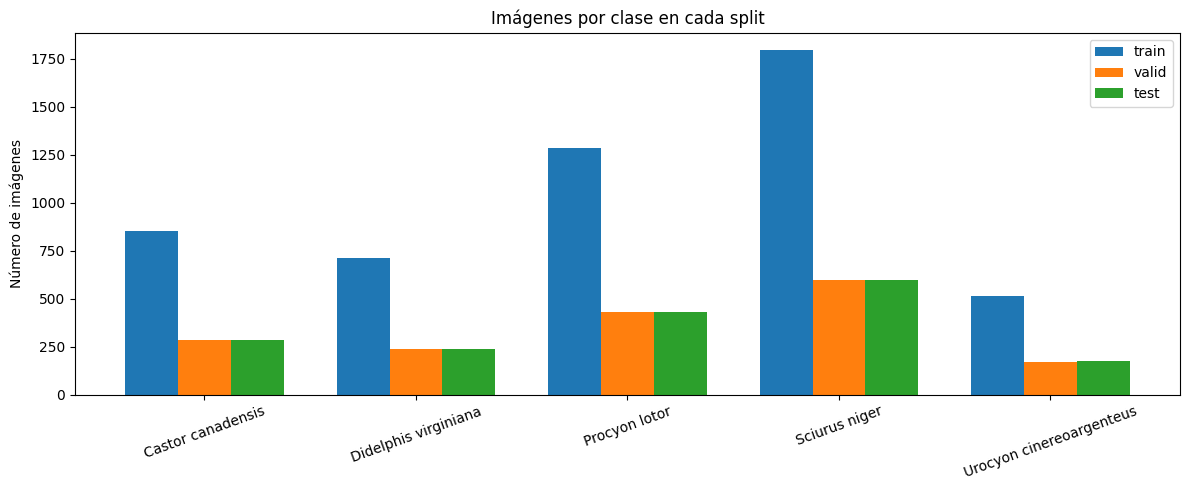
\includegraphics[width=0.95\textwidth]{figs/conteo_clases.png}
\caption{Número de imágenes por clase en los conjuntos de entrenamiento, validación y prueba.}
\label{fig:conteo}
\end{figure}

\subsection{Distribución de los datos entre conjuntos}

El conjunto completo tiene 8610 imágenes, repartidas en 60\,\% para entrenamiento (5163), 20\,\% para validación (1723) y 20\,\% para prueba (1724). Esta proporción 60/20/20 se mantiene dentro de cada clase, por lo que la partición es estratificada: la proporción de cada especie es la misma en los tres conjuntos y los resultados de validación y prueba serán representativos de la distribución de entrenamiento.

Sin embargo, las clases no están balanceadas entre sí. \emph{Sciurus niger} es la clase mayoritaria, con el 34,8\,\% de las imágenes, mientras que \emph{Urocyon cinereoargenteus} es la minoritaria, con el 10,0\,\%. La relación entre la clase más grande y la más pequeña es de aproximadamente 3,5 a 1. Este desbalance debe tenerse en cuenta en las siguientes entregas: un clasificador podría favorecer a las clases mayoritarias, por lo que conviene evaluar con métricas que no dependan de la frecuencia de cada clase (por ejemplo, precisión y cobertura por clase, o F1 promedio) y considerar estrategias como el submuestreo, el aumento de datos de las clases minoritarias o la ponderación de clases.

\subsection{Ejemplos visuales}

La Figura~\ref{fig:ejemplos} muestra una imagen tomada al azar de cada clase en cada conjunto. Los ejemplos ilustran la gran variabilidad del conjunto de datos, que es una de las principales dificultades de la tarea:

\begin{itemize}
  \item \textbf{Rastros en lugar de animales:} algunas imágenes no muestran al animal sino sus huellas, como el castor en entrenamiento o el mapache en validación.
  \item \textbf{Animales pequeños dentro del encuadre:} en varias fotografías el animal ocupa una fracción muy pequeña de la imagen, como el mapache y el zorro gris en entrenamiento o el castor en validación.
  \item \textbf{Camuflaje y oclusión:} el fondo (hojas, ramas, tierra) se confunde con el animal, como ocurre con la ardilla zorro en validación y prueba.
  \item \textbf{Animales muertos:} aparecen animales atropellados en la carretera, como el castor y el zorro gris en prueba, cuya apariencia difiere mucho de la de un animal vivo.
  \item \textbf{Condiciones de captura variables:} hay fotografías nocturnas, a contraluz, con distintos encuadres y con personas en la escena.
\end{itemize}

\begin{figure}[H]
\centering
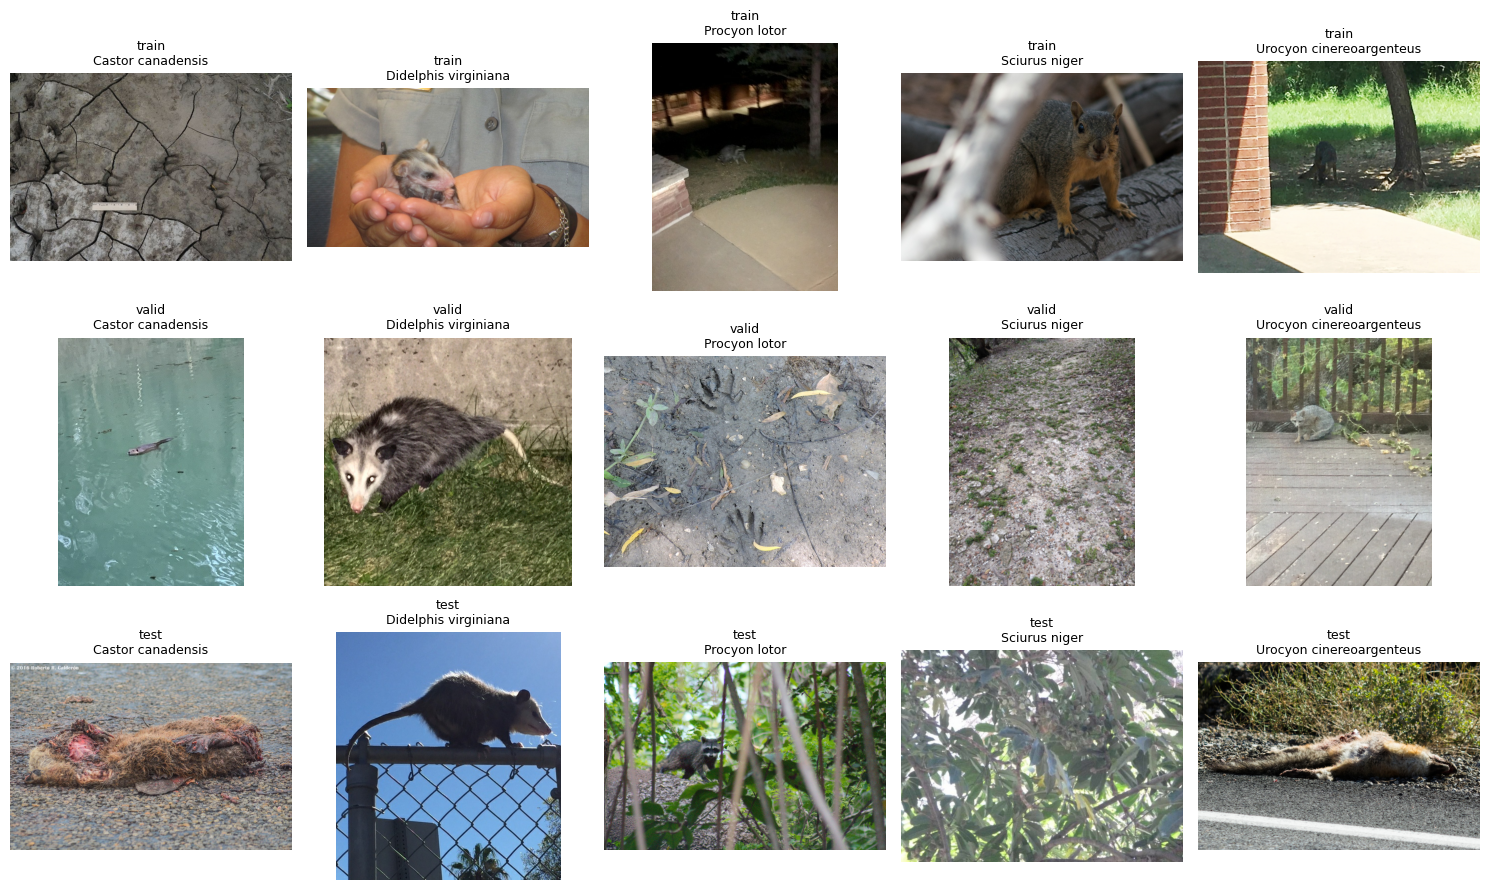
\includegraphics[width=\textwidth]{figs/ejemplos.png}
\caption{Una imagen aleatoria de cada clase (columnas) en cada conjunto (filas: entrenamiento, validación y prueba).}
\label{fig:ejemplos}
\end{figure}

\subsection{Otras estadísticas}

Se leyeron las 8610 imágenes para obtener estadísticas de tamaño y color:

\begin{itemize}
  \item \textbf{Imágenes corruptas:} ninguna. Todas las imágenes se pudieron leer con \texttt{cv2.imread}.
  \item \textbf{Imágenes en escala de grises:} 124 de 8610 (1,4\,\%). Como \texttt{cv2.imread} siempre devuelve tres canales, una imagen se consideró en escala de grises cuando sus tres canales son idénticos.
  \item \textbf{Alto:} mínimo 121 píxeles, máximo 800 y promedio 613,4.
  \item \textbf{Ancho:} mínimo 148 píxeles, máximo 800 y promedio 686,6.
\end{itemize}

La Figura~\ref{fig:tamanos} muestra los histogramas de alto y ancho. Ninguna dimensión supera los 800 píxeles y se observan picos en 600 y 800, lo que indica que las imágenes ya fueron reescaladas para que su lado mayor no exceda los 800 píxeles. Aun así, los tamaños y las relaciones de aspecto son variados, lo que justifica redimensionar todas las imágenes a un tamaño fijo antes de extraer descriptores. La presencia de imágenes en escala de grises, aunque minoritaria, es relevante para los descriptores de color, que en esas imágenes no aportan información de tono.

\begin{figure}[H]
\centering
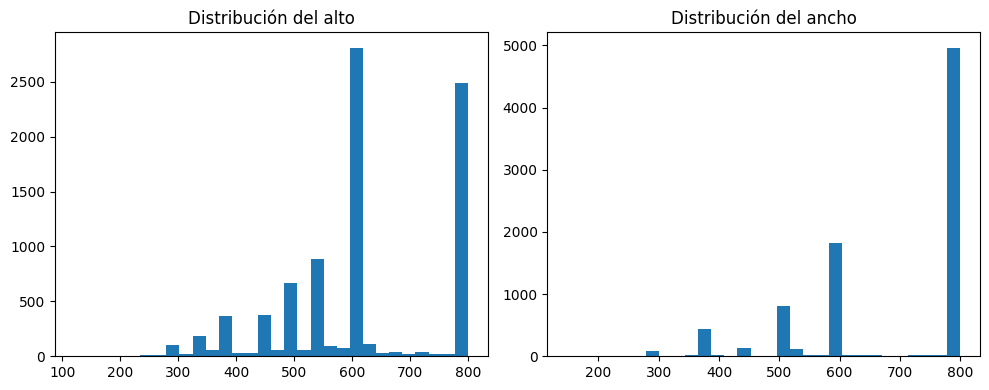
\includegraphics[width=0.85\textwidth]{figs/tamanos.png}
\caption{Distribución del alto (izquierda) y del ancho (derecha) de las imágenes, en píxeles.}
\label{fig:tamanos}
\end{figure}

\section{Preprocesamiento de las imágenes}

\subsection{Preprocesamientos básicos}

La función \texttt{processing} aplica dos transformaciones opcionales usando únicamente funciones de OpenCV. Primero redimensiona la imagen con \texttt{cv2.resize} si se especifica \texttt{img\_size}, y después la convierte del espacio BGR (el formato en que \texttt{cv2.imread} lee las imágenes) al espacio de color pedido con \texttt{cv2.cvtColor}. Si alguno de los parámetros es \texttt{None}, la transformación correspondiente no se aplica.

\begin{lstlisting}
if img_size is not None:
    Im = cv2.resize(Im, img_size)

if color_space is not None:
    conversions = {"rgb": cv2.COLOR_BGR2RGB, "gray": cv2.COLOR_BGR2GRAY,
                   "hsv": cv2.COLOR_BGR2HSV, "lab": cv2.COLOR_BGR2LAB}
    Im = cv2.cvtColor(Im, conversions[color_space])
\end{lstlisting}

El orden (primero redimensionar y luego convertir) coincide con el que usan las pruebas. La función superó todas las verificaciones: tamaño $224\times224$ en RGB, escala de grises (un solo canal), HSV y Lab; tamaño $256\times256$ sin cambio de color; y conversión a Lab sin redimensionar.

\subsection{Data augmentation}

La función \texttt{data\_augmentation} implementa tres transformaciones:

\begin{itemize}
  \item \textbf{Reflejo horizontal (\texttt{flip}):} refleja la imagen respecto al eje $y$ con \texttt{cv2.flip(Im, 1)}.
  \item \textbf{Contraste (\texttt{contrast}):} multiplica la intensidad por un factor $\alpha$ tomado de una distribución uniforme en el rango \texttt{alpha\_factor}, con $\beta=0$.
  \item \textbf{Brillo (\texttt{brightness}):} suma a la intensidad un valor $\beta$ tomado de una distribución uniforme en el rango \texttt{beta\_factor}, con $\alpha=1$.
\end{itemize}

Las tres operaciones de intensidad usan \texttt{cv2.convertScaleAbs}, que calcula $g(x) = |\alpha f(x) + \beta|$ y satura el resultado al rango $[0, 255]$. Cuando se piden brillo y contraste al mismo tiempo (\texttt{"brightness and contrast"}), se generan primero $\alpha$ y luego $\beta$, y se aplican en una sola llamada a \texttt{convertScaleAbs}, como indica el enunciado. Los valores aleatorios se generan con \texttt{random.uniform} para que la semilla fijada en las pruebas (\texttt{random.seed(1)}) produzca resultados reproducibles.

La Figura~\ref{fig:aug} muestra el resultado de las cuatro combinaciones probadas sobre una imagen de \emph{Castor canadensis}, con $\alpha \in [1{,}5;\ 2{,}5]$ y $\beta \in [20;\ 80]$.

\begin{figure}[H]
\centering
\begin{subfigure}{0.49\textwidth}
  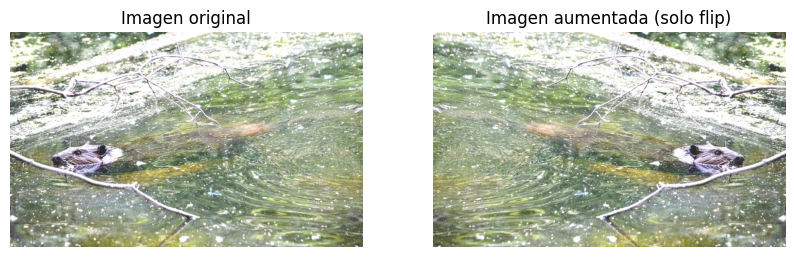
\includegraphics[width=\textwidth]{figs/aug_flip.png}
  \caption{Solo reflejo horizontal.}
\end{subfigure}
\hfill
\begin{subfigure}{0.49\textwidth}
  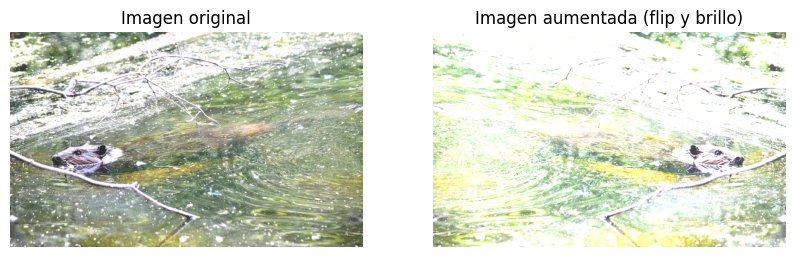
\includegraphics[width=\textwidth]{figs/aug_contraste.png}
  \caption{Reflejo y contraste ($\alpha \in [1{,}5;\ 2{,}5]$).}
\end{subfigure}

\vspace{0.5em}
\begin{subfigure}{0.49\textwidth}
  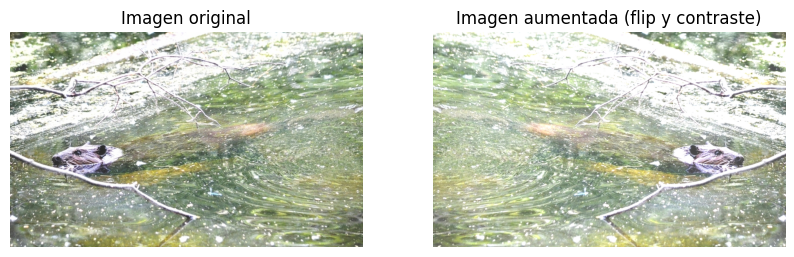
\includegraphics[width=\textwidth]{figs/aug_brillo.png}
  \caption{Reflejo y brillo ($\beta \in [20;\ 80]$).}
\end{subfigure}
\hfill
\begin{subfigure}{0.49\textwidth}
  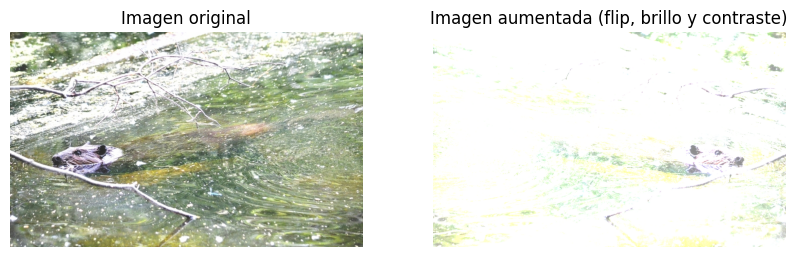
\includegraphics[width=\textwidth]{figs/aug_brillo_contraste.png}
  \caption{Reflejo, brillo y contraste.}
\end{subfigure}
\caption{Resultados de \emph{data augmentation}. En cada panel, la imagen original está a la izquierda y la aumentada a la derecha. Los títulos internos de los paneles (b) y (c) provienen de la plantilla del notebook y están intercambiados: el panel (b) corresponde al ajuste de contraste y el (c) al de brillo.}
\label{fig:aug}
\end{figure}

Se observa que el reflejo conserva toda la información de la imagen y solo invierte la orientación del animal. El ajuste de brillo con $\beta \in [20;\ 80]$ produce un cambio moderado. En cambio, el contraste con $\alpha \in [1{,}5;\ 2{,}5]$ satura gran parte de los píxeles a 255, y la combinación de brillo y contraste deja la imagen casi blanca, con el castor apenas visible. Esto ocurre porque la imagen original ya es muy clara. Para usar el aumento de datos en el entrenamiento convendría emplear rangos más suaves (por ejemplo, $\alpha \in [0{,}8;\ 1{,}2]$ y $\beta \in [-30;\ 30]$), de modo que las imágenes generadas sigan siendo realistas.

\section{Conclusiones}

\begin{itemize}
  \item Se completaron todas las secciones de código del notebook y todas las pruebas automáticas se superaron.
  \item El subconjunto asignado al grupo 19 tiene 8610 imágenes de cinco especies, con una partición estratificada 60/20/20 y un desbalance entre clases de aproximadamente 3,5 a 1, que deberá considerarse al entrenar y evaluar los clasificadores.
  \item Las imágenes presentan una gran variabilidad (rastros, animales muy pequeños, camuflaje, animales muertos y condiciones de captura diversas), lo que anticipa que la clasificación con descriptores clásicos será un problema difícil.
  \item Las imágenes tienen tamaños variados con un máximo de 800 píxeles y un 1,4\,\% está en escala de grises, lo que justifica redimensionar a un tamaño fijo y tener cuidado con los descriptores de color.
  \item Las funciones de preprocesamiento y aumento de datos quedaron listas para las siguientes entregas. Los rangos de brillo y contraste usados en las pruebas son agresivos y deberían suavizarse al aplicarlos en el entrenamiento.
\end{itemize}

\end{document}
